\documentclass[tikz, border=5pt]{standalone}
\usetikzlibrary{arrows.meta}
\usetikzlibrary{decorations.markings}
    
    \newcommand{\xmarker}[2]{%
      \draw[thin,#2] (-#1,-#1)--(#1,#1);
      \draw[thin,#2] (-#1,#1)--(#1,-#1);
    }
\begin{document}
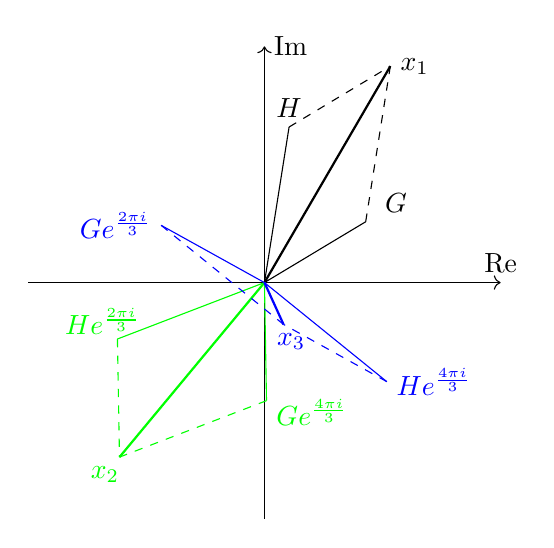
\begin{tikzpicture}
  \def\H{2.0}
  \def\G{1.5}
  \def\phiH{81}
  \def\phiG{31}
  \def\l{3}
  \draw [->](-\l, 0)--(\l, 0) node [above]{Re};
  \draw [->](0,-\l)--(0, \l) node [right]{Im};
  \draw (0,0)--({cos(\phiH)*\H}, {sin(\phiH)*\H}) node[pos=1, above] {$H$};
  \draw (0,0)--({cos(\phiG)*\G}, {sin(\phiG)*\G}) node[pos=1.3] {$G$};
  \draw [thick](0,0) -- ({cos(\phiH)*\H+cos(\phiG)*\G}, {sin(\phiH)*\H+sin(\phiG)*\G}) node[pos=1, right]{$x_1$};
  \draw [dashed]({cos(\phiH)*\H}, {sin(\phiH)*\H})--({cos(\phiH)*\H+cos(\phiG)*\G}, {sin(\phiH)*\H+sin(\phiG)*\G});
  \draw [dashed]({cos(\phiG)*\G}, {sin(\phiG)*\G})--({cos(\phiH)*\H+cos(\phiG)*\G}, {sin(\phiH)*\H+sin(\phiG)*\G});

  \draw [green](0,0)--({cos(\phiH+120)*\H}, {sin(\phiH+120)*\H}) node[pos=1.1, above,text=green] {$He^{\frac{2\pi i}{3}}$};
  \draw [green](0,0)--({cos(\phiG+240)*\G}, {sin(\phiG+240)*\G}) node[pos=1.1, right,text=green] {$Ge^{\frac{4\pi i}{3}}$};
  \draw [green,thick](0,0) -- ({cos(\phiH+120)*\H+cos(\phiG+240)*\G}, {sin(\phiH+120)*\H+sin(\phiG+240)*\G}) node[pos=1.1, text=green]{$x_2$};
  \draw [green,dashed]({cos(\phiH+120)*\H}, {sin(\phiH+120)*\H})--({cos(\phiH+120)*\H+cos(\phiG+240)*\G}, {sin(\phiH+120)*\H+sin(\phiG+240)*\G});
  \draw [green,dashed]({cos(\phiG+240)*\G}, {sin(\phiG+240)*\G})--({cos(\phiH+120)*\H+cos(\phiG+240)*\G}, {sin(\phiH+120)*\H+sin(\phiG+240)*\G});

  \draw [blue](0,0)--({cos(\phiH+240)*\H}, {sin(\phiH+240)*\H}) node[pos=1, right, text=blue] {$He^{\frac{4\pi i}{3}}$};
  \draw [blue](0,0)--({cos(\phiG+120)*\G}, {sin(\phiG+120)*\G}) node[pos=1, left, text=blue] {$Ge^{\frac{2\pi i}{3}}$};
  \draw [blue,thick](0,0) -- ({cos(\phiH+240)*\H+cos(\phiG+120)*\G}, {sin(\phiH+240)*\H+sin(\phiG+120)*\G}) node[pos=1.4,  text=blue]{$x_3$};
  \draw [blue,dashed]({cos(\phiH+240)*\H}, {sin(\phiH+240)*\H})--({cos(\phiH+240)*\H+cos(\phiG+120)*\G}, {sin(\phiH+240)*\H+sin(\phiG+120)*\G});
  \draw [blue,dashed]({cos(\phiG+120)*\G}, {sin(\phiG+120)*\G})--({cos(\phiH+240)*\H+cos(\phiG+120)*\G}, {sin(\phiH+240)*\H+sin(\phiG+120)*\G});
  

\end{tikzpicture}
\end{document}

